
\vspace{-5mm}
\section{Theory}
	When a coherent light beam is passed through a thin wire or slit with a thickness comparable to the wavelength of the light, a phenomenon known as diffraction occurs. This interference pattern on a distant screen is caused by secondary waves from the emerging beam's wavefront, which have a constant phase difference as they arrive at the screen by travelling different distances. Fraunhofer diffraction is the name given to this type of diffraction, in which the light source, the screen, and the object causing the diffraction are all practically at an infinite distance from one another. The slit width is on par with the light's wavelength. We will investigate Franhouffer diffraction in the experiment, which is caused by diffraction through single, double, and narrow wires.

	\vspace{-5mm}
	\subsection{Single Slit Diffraction}
		For single-slit diffraction, the intensity of the transmitted light on the screen is given by:

		$$I = I_0 \frac{\sin\beta^2}{\beta^2}$$

		Where $\beta = \frac{\pi b\sin\theta}{\lambda}$, b is the width of the slit. For minima $\beta = m\pi$, where m is set of integers. Therefore, the condition for minima is: $m\lambda = b \sin\theta$. For small angle of inclination (for larger distance between the source, slit and screen, $\theta\approx\sin\theta\approx\tan\theta=\frac{x}{2D}$ where x is distance between corresponding m-th minimas on both side of the principle maxima and D is distance between the slit and the screen).

		\vspace{2cm}
		Therefore we get:

		\begin{equation}
			x = \frac{2Dm\lambda}{b}
			\label{eqn:1}
		\end{equation}

		\begin{figure}[H]
			\centering
			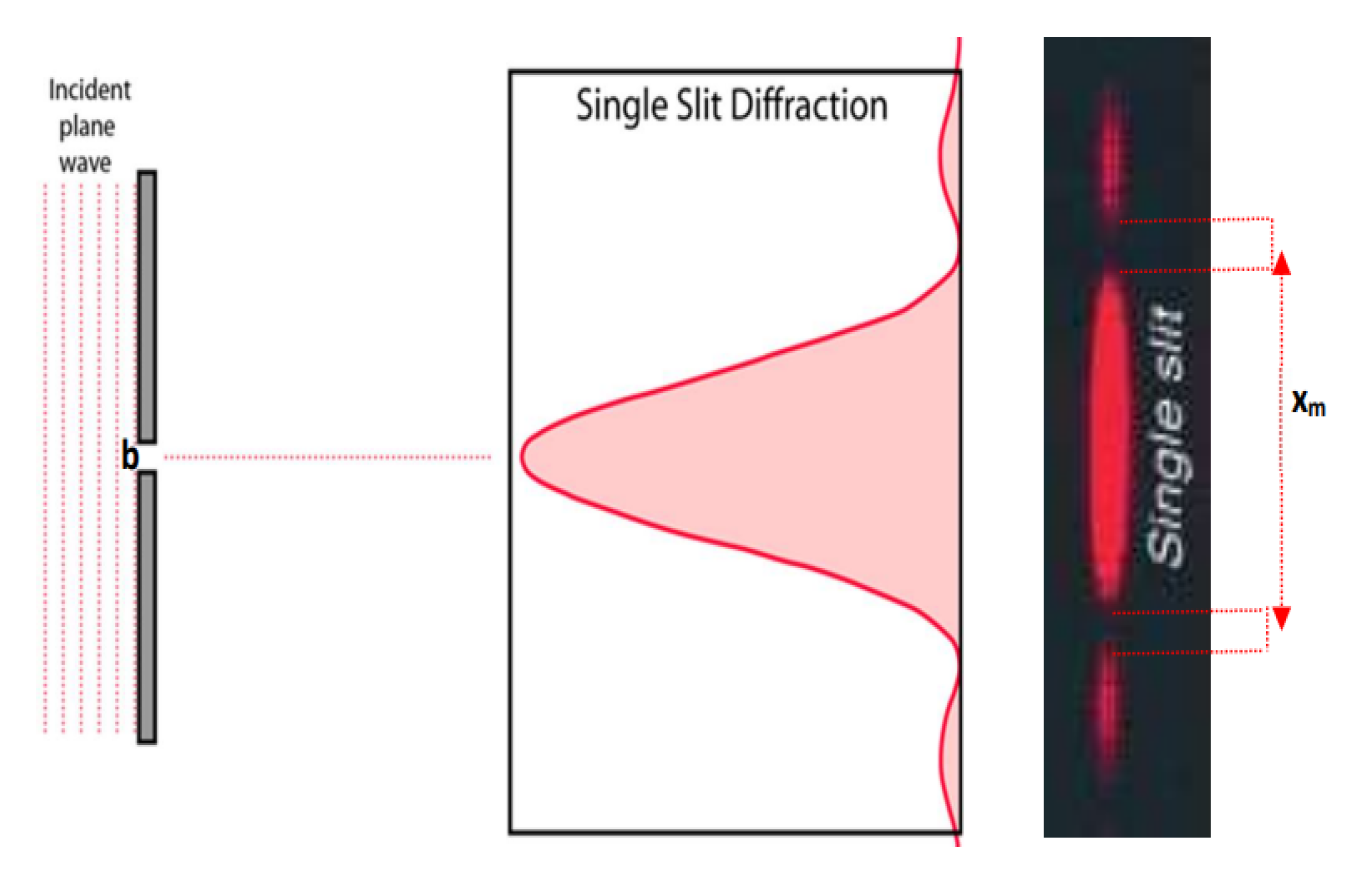
\includegraphics[width=0.4\textwidth]{images/single_slit.png}
			\caption{Schematics of Single Slit Diffraction}
			\label{fig:1}
		\end{figure}

		\begin{figure}[H]
			\centering
			\includegraphics[width=0.4\textwidth]{images/photo_1.png}
			% \caption{Schematics of Single Slit Diffraction}
			\label{pic:1}
		\end{figure}

	\subsection{Diffraction of thin wire}
		A similar diffraction pattern to that of a single slit is obtained on the screen when the single-slit is replaced by a wire that blocks light with an equal amount of intensity as the single slit. Therefore, the following is the relationship between the minimas and inclination:

		\begin{equation}
			x = \frac{2Dm\lambda}{\pi d}
			\label{eqn:2}
		\end{equation}

		The general rule known as \textbf{Babinet's principle} is illustrated by the fact that the Fraunhofer diffraction pattern caused by an obstruction is almost identical to that of an opening of the same dimension. This idea can be tested by replacing the wire with a single slit once more and adjusting the slit width until the pattern is perfectly uniform. The slit width and wire thickness can then be compared.
	
	\subsection{Double slit Diffraction \& Interference}
		The distance between the centres of the two slits is d(= c+b), and a double slit is made up of two openings of width b and an opaque region between them of width c. The diffraction patterns from the two slits interfere on the screen as the light beam travels through the slits. The following factors determine the intensity of the corresponding Franhouffer pattern:

		$$I = I_0 \frac{\sin\beta^2}{\beta^2} \cos\gamma^2$$
		$$\beta = \frac{\pi b\sin\theta}{\lambda}$$
		$$\gamma = \frac{\pi d\sin\theta}{\lambda}$$

		Where the $\sin\beta^2$ represents the diffraction pattern produced by the single-slit and the second term $\cos\gamma^2$ is the characteristic of interference produced by two beams of equal intensity and phase difference $\gamma$. The overall pattern, therefore, consists of single-slit diffraction fringes each broken into narrow maxima and minima of interference fringe. The conditions for minima are:

		$$d\sin\theta = (p+0.5)\lambda$$
		$$b\sin\theta = m\lambda$$

		\begin{figure}[H]
			\centering
			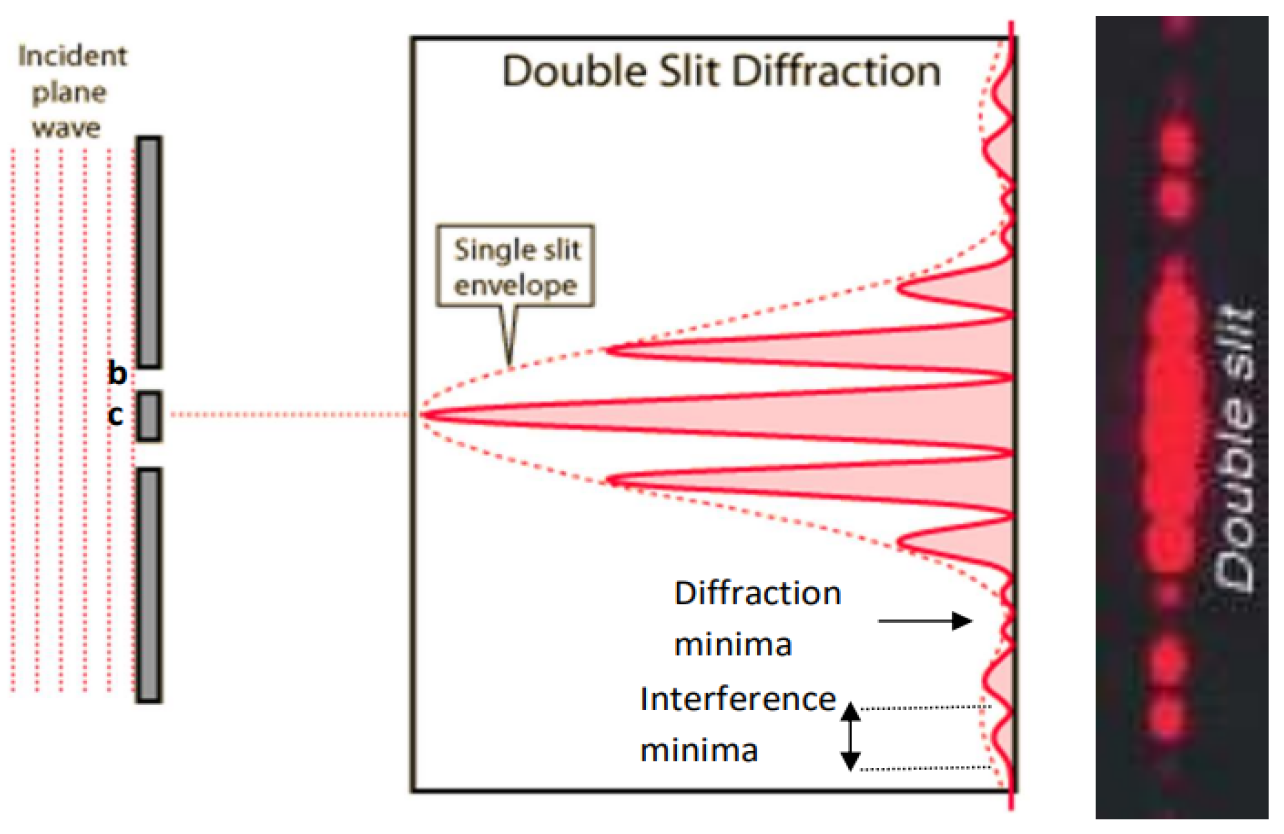
\includegraphics[width=0.4\textwidth]{images/double_slit.png}
			\caption{Schematics of Double Slit Diffraction}
			\label{fig:2}
		\end{figure}

		\begin{figure}[H]
			\centering
			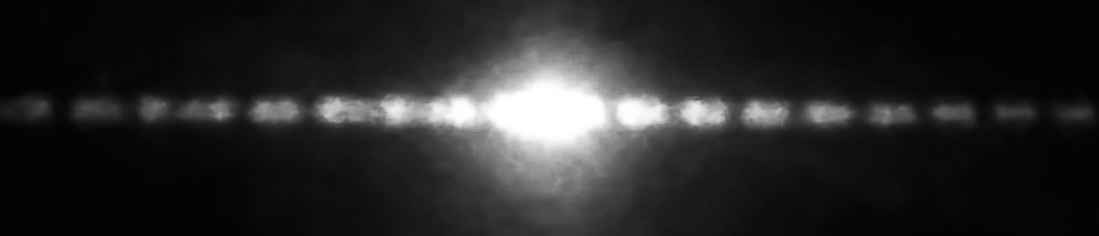
\includegraphics[width=0.4\textwidth]{images/photo_2.png}
			% \caption{Schematics of Single Slit Diffraction}
			\label{pic:2}
		\end{figure}

		Instead of calculating the distance between the corresponding minimas on both sides, we will calculate the distance between n minimas on each side and average them because it is difficult to determine the order of the interference and diffraction pattern. Let the distance of $(m+n)$th diffraction minima from the central maxima be $x_{m+n}$ and for $m^th$ minima be $x_m$, then the distance between the minimas is: $\Delta x_m = x_{m+n} - x_m$. Similarly for the interference minima, the distance between $n$ minimas is: $\Delta x_p = x_{p+n} - x_p$. For large distance the relation between the angle of inclination and the distance is given by:

		\begin{equation}
			\frac{n}{\Delta x_p} = \frac{d}{D\lambda}
			\label{eqn:3}
		\end{equation}

		\begin{equation}
			\frac{n}{\Delta x_m} = \frac{b}{D\lambda}
			\label{eqn:4}
		\end{equation}

